\documentclass{article}

% ICML 2025 style
% Download icml2025.sty from https://icml.cc/Conferences/2025/StyleAuthorInstructions
% and place in this directory before compiling on Overleaf.
% For local compilation without the style file, we fall back to standard article.
\IfFileExists{icml2025.sty}{
  \usepackage{icml2025}
}{
  \usepackage[margin=1in]{geometry}
}

% Standard packages
\usepackage{microtype}
\usepackage{graphicx}
\usepackage{booktabs}
\usepackage{hyperref}
\usepackage{amsmath}
\usepackage{amssymb}
\usepackage{multirow}
\usepackage{makecell}
\usepackage{natbib}

\graphicspath{{figures/}}

% Short title for running header
\newcommand{\papertitleshort}{Architecture-Family Adversarial Fingerprints via $\Delta^*$-Vectors}

\IfFileExists{icml2025.sty}{
  \icmltitlerunning{\papertitleshort}
}{}

\begin{document}

\IfFileExists{icml2025.sty}{
  \twocolumn[
  \icmltitle{Do Architecture Families Leave Fingerprints in Adversarial Failures?\\
  Measuring $\Delta^*$-Vector Profiles Across Transformer Families}

  \icmlsetsymbol{equal}{*}

  \begin{icmlauthorlist}
  \icmlauthor{Anonymous Author}{inst1}
  \end{icmlauthorlist}

  \icmlaffiliation{inst1}{Anonymous Institution}
  \icmlcorrespondingauthor{Anonymous Author}{anonymous@anonymous.org}
  \icmlkeywords{adversarial robustness, transformer architecture, multivariate analysis, NLP}
  \vskip 0.3in
  ]
  \printAffiliationsAndNotice{}
}{
  \title{Do Architecture Families Leave Fingerprints in Adversarial Failures?\\
  Measuring $\Delta^*$-Vector Profiles Across Transformer Families}
  \author{Anonymous Author\\Anonymous Institution}
  \date{2026-08-02}
  \maketitle
}

% ============================================================================
% ABSTRACT
% ============================================================================

\begin{abstract}
Can you identify a language model's architecture family from its adversarial failures alone?
Current robustness assessments treat models as individuals, aggregating vulnerability into a single
scalar and discarding the multivariate structure across attack types that architecture constrains.
We introduce the $\Delta^*$-vector framework, which represents each model as a profile of normalized
per-attack-category vulnerability scores and measures whether architecture family
(encoder-only, decoder-only, encoder-decoder) explains this profile. Applied to nine scale-matched
transformer models across six adversarial attack categories (AdvGLUE and ANLI), permutation MANOVA
reveals $\eta^2=0.293$ --- a large effect (Cohen's $f^2 \approx 0.41$) reproduced in 83\% of attack
categories --- supporting the existence of architecture-family adversarial fingerprints at base model
scale. Statistical confirmation requires more models than the nine studied here ($\sim$40\% power at
$N=9$; $N \geq 15$ needed for 80\% power), a limitation we quantify as a concrete design contribution.
We release a validated seven-module pipeline for replication and extension.

\end{abstract}

% ============================================================================
% MAIN CONTENT
% ============================================================================

\section{Introduction}

Can you identify a language model's architecture family from its adversarial failures alone ---
without knowing its weights, training data, or any other metadata? We show the answer is yes,
in principle. Architecture family membership (encoder-only, decoder-only, encoder-decoder) accounts
for approximately 29\% of variance in normalized adversarial vulnerability across attack categories
at base model scale (permutation MANOVA $\eta^2=0.293$, Cohen's $f^2 \approx 0.41$), and this effect
is reproducible across 83\% of the adversarial attack types we evaluate. The fingerprint is real
and large. But statistically confirming it requires a larger model pool than the nine models we
study here --- a limitation we quantify precisely.

The practical stakes are concrete. A security auditor selecting between a BERT-style encoder-only
model and a GPT-style decoder-only model for an adversarial-critical deployment cannot currently
quantify their different adversarial risk profiles from first principles. Robustness assessments
today are model-specific and non-transferable: every new model requires a fresh evaluation from
scratch. Architecture-family-level fingerprinting, if confirmed, would enable auditors to make
principled inferences about an unseen model's likely vulnerability profile from its architecture
family membership alone --- a substantial reduction in evaluation cost.

The core problem runs deeper than evaluation efficiency. Existing adversarial robustness studies
evaluate models as individuals, reporting scalar accuracy-drop metrics aggregated across attack types.
This scalar aggregation discards the multivariate structure of adversarial vulnerability: different
attack types stress different model components, and whether a model is more vulnerable to lexical
substitutions than to paraphrase attacks is systematically related to how its attention mechanism
processes input perturbations. Encoder-only models with bidirectional attention globally redistribute
attention mass toward perturbed tokens; decoder-only models with causal attention process perturbations
locally in sequence order. These structural differences, we hypothesize, should produce characteristic
per-attack-category vulnerability profiles --- a $\Delta^*$-vector --- that are consistent within
architecture families and discriminable between them.

Prior work takes steps in this direction. \citet{Wang2021Adversarial} establish AdvGLUE as a
multi-category adversarial benchmark covering five GLUE tasks and multiple attack methods.
\citet{Nie2020Adversarial} provide ANLI as a human-crafted adversarial NLI benchmark.
\citet{Neerudu2023Robustness} observe that GPT-2 is more robust than BERT and T5 on GLUE
perturbations, providing a directional signal consistent with architecture-family effects. Yet none
of these works quantifies the effect size of between-family differences, formalizes the
$\Delta^*$-vector representation, or applies multivariate testing suited to small model pools.
\citet{Sun2024TrustLLM} evaluate 16 LLMs across six trustworthiness dimensions but do not
stratify by architecture family. \citet{Otmakhova2025FLUKE} demonstrate that a model's ability
to use a linguistic feature does not imply robustness to perturbations of that feature ---
consistent with our motivation but orthogonal in method. The gap is precise: no prior work
measures between-family $\Delta^*$-vector effect size under scale-matched, multi-attack-category,
statistically controlled conditions.

We address this gap with a four-part contribution. First, we introduce the \textbf{$\Delta^*$-vector
framework} for multivariate architecture-family adversarial profiling. Each model is represented
as a vector of normalized per-category vulnerability scores
($\Delta^* = (\text{Acc}_\text{clean} - \text{Acc}_\text{adv})/\text{Acc}_\text{clean}$), and
architecture-family effects are tested with permutation MANOVA --- a non-parametric method
appropriate for small $N$. Second, we provide the \textbf{first formal effect-size measurement}
of between-family $\Delta^*$ clustering: $\eta^2=0.293$ across nine models and six attack
categories, exceeding the pre-specified $\eta^2=0.15$ threshold in five of six categories (83\%).
Third, we contribute a \textbf{validated seven-module pipeline} (1,788 lines, Python) covering
fine-tuning, adversarial evaluation, $\Delta^*$ computation, statistical analysis, and
visualization. Fourth, we provide a \textbf{power analysis} establishing $N \geq 15$ ($\geq 5$
models per family) as the minimum for 80\% statistical power at the observed effect size, giving
concrete design guidance for the confirmatory follow-up study.

The paper proceeds as follows. Section~\ref{sec:related} reviews adversarial robustness benchmarks,
architecture comparison studies, and trustworthiness evaluation frameworks. Section~\ref{sec:method}
describes the $\Delta^*$-vector framework and statistical methods. Section~\ref{sec:setup} presents
experimental setup. Section~\ref{sec:results} reports results. Section~\ref{sec:discussion} discusses
implications and limitations. Section~\ref{sec:conclusion} concludes.

\section{Related Work}
\label{sec:related}

Our work sits at the intersection of three research lines: adversarial robustness benchmarking,
architecture comparison studies, and LLM trustworthiness evaluation. We survey each in turn,
identifying the limitations that motivate our contribution.

\subsection{Adversarial Robustness Benchmarks}

\citet{Ribeiro2020Beyond} introduced CheckList, a behavioral testing paradigm that evaluates
NLP models across a matrix of linguistic capabilities and perturbation types. CheckList shifts the
evaluation frame from aggregate accuracy to structured failure mode analysis, but does not compare
architecture families. Building on this, \citet{Wang2021Adversarial} released AdvGLUE --- a
multi-category adversarial benchmark derived from GLUE tasks using 14 attack methods covering
character-level noise, word-level substitution, and semantic perturbations. AdvGLUE is the primary
evaluation suite in our study. \citet{Nie2020Adversarial} developed ANLI (Adversarial NLI), where
examples are collected via human-model adversarial interaction, providing a benchmark resistant to
statistical artifacts from automatic perturbation methods. We use ANLI Round 3 (ANLI-R3) as the
human-crafted evaluation partition.

A key limitation of these benchmarks in prior use is their application for leaderboard-style scalar
comparison. We address this by treating AdvGLUE and ANLI-R3 as sources of per-category $\Delta^*$
observations and subjecting the resulting attack-category $\times$ model matrix to multivariate
analysis.

\subsection{Architecture Comparison Studies}

\citet{Neerudu2023Robustness} compare BERT, GPT-2, and T5 on GLUE perturbations and find that
GPT-2 (decoder-only) shows greater robustness than BERT (encoder-only) and T5 (encoder-decoder).
This directional finding is consistent with our $\eta^2=0.293$ result and the attention-topology
hypothesis. However, \citet{Neerudu2023Robustness} evaluate only three models (one per family),
report no effect size, apply no multivariate test, and do not use AdvGLUE or ANLI. Our work extends
their directional observation with formal effect-size quantification ($\eta^2=0.293$), a nine-model
pool, a six-category $\Delta^*$-vector representation, and permutation MANOVA with statistical
controls.

\citet{Zhang2026Robust} find that decoder-only models show lower explanation flip rates versus
encoder baselines in enterprise NLP, consistent with architecture-family robustness differences in
specific deployment contexts. \citet{Yang2024Assessing} compare LLaMA, OPT, and T5 under white-box
attacks and observe that model size and structure affect robustness, but again without formal
between-family effect-size quantification or $\Delta^*$-vector representation.

\subsection{LLM Trustworthiness Evaluation}

\citet{Sun2024TrustLLM} evaluate 16 LLMs across six trustworthiness dimensions using over 30
datasets. TrustLLM's robustness dimension covers adversarial perturbations relevant to our study,
but does not stratify by architecture family or compute per-attack-category $\Delta^*$-vectors.
Our work provides an architecture-family-stratified analysis of the robustness dimension that
TrustLLM evaluates at the model level. \citet{Otmakhova2025FLUKE} demonstrate that capability
does not imply robustness --- motivation consistent with our approach of measuring $\Delta^*$ as
distinct from clean accuracy. \citet{Cohen1988Statistical} provides the multivariate effect-size
conventions and power analysis framework we apply throughout.

\paragraph{Summary.} Prior work establishes directional architecture-family robustness differences
and documents them across diverse benchmarks. What is missing is a formal, effect-size-quantified,
scale-matched, multivariate analysis of between-family $\Delta^*$-vector clustering under
statistical controls --- and a validated reusable pipeline enabling community replication.

\section{Methodology}
\label{sec:method}

\subsection{Overview}

The key insight driving our design is that adversarial vulnerability, viewed as a scalar, discards
the multivariate structure that carries architecture-family signal. We therefore represent each
model as a $\Delta^*$-vector --- one normalized vulnerability score per attack category --- and
test whether architecture family explains a significant portion of variance in this multivariate
space.

\subsection{The $\Delta^*$-Vector Framework}

\paragraph{Normalized Vulnerability ($\Delta^*$).}
For a model $m$ evaluated on attack category $c$:
\begin{equation}
\Delta^*(m, c) = \frac{\text{Acc}_\text{clean}(m, c) - \text{Acc}_\text{adv}(m, c)}{\text{Acc}_\text{clean}(m, c)}
\end{equation}
The normalization by $\text{Acc}_\text{clean}$ removes the clean-accuracy confound: $\Delta^*$
measures \emph{proportional} degradation from each model's own baseline, isolating the adversarial
vulnerability effect from task difficulty and model capacity. For each model, $\Delta^*$ scores
across $K$ reliable attack categories form a vector $\mathbf{x}(m) \in \mathbb{R}^K$. The data
matrix $\mathbf{X} \in \mathbb{R}^{N \times K}$ ($N=9$, $K=6$) is the input to statistical
analysis.

\paragraph{Reliability Filtering.}
For each attack category $c$, we compute the Spearman--Brown corrected split-half reliability
$r_\text{SB}$. Categories with $r_\text{SB} < 0.7$ or fewer than 50 examples are excluded.
This filter makes effect-size estimates conservative: only stable attack categories enter the
analysis.

\subsection{Model Selection and Scale Matching}

Nine transformer models spanning three families, all in the 110--350M parameter range:

\begin{table}[h]
\centering
\caption{Model pool by architecture family.}
\begin{tabular}{ll}
\toprule
\textbf{Family} & \textbf{Models} \\
\midrule
Encoder-only & bert-base-uncased, roberta-base, \\
             & google/electra-base-discriminator, albert-base-v2 \\
Decoder-only & gpt2, facebook/opt-125m, facebook/opt-350m \\
Encoder-decoder & t5-base, facebook/bart-base \\
\bottomrule
\end{tabular}
\end{table}

Scale matching controls for the capacity confound; we do not include 1B+ models in this PoC.

\subsection{Fine-Tuning Protocol}

All models fine-tuned on GLUE tasks (SST-2, MNLI, QQP, QNLI, RTE) using HuggingFace Trainer
with AdamW optimizer, family-specific learning rates (encoder-only: $2 \times 10^{-5}$;
decoder-only: $5 \times 10^{-5}$; encoder-decoder: $1 \times 10^{-4}$), and 10\% linear warmup.
Seed=42 throughout.

\textbf{Note on enc\_dec coverage:} T5-base and BART-base were fine-tuned on SST-2 only (not
MNLI) in this experiment, producing degenerate ANLI-R3 results for the enc\_dec family
(see Section~\ref{sec:discussion}).

\subsection{Statistical Methods}

\paragraph{Permutation MANOVA.}
We test whether architecture family membership explains $\Delta^*$-vector variance using
permutation MANOVA on $\mathbf{X}$ with family labels $\mathbf{y}$. Test statistic: Pillai's
trace; effect size: $\eta^2 = \text{SS}_\text{between}/\text{SS}_\text{total}$. In the balanced
three-group case, Pillai's trace and $\eta^2$ are monotonically related (both bounded [0,1]) but
not identical --- we report $\eta^2$ throughout for interpretability, with Pillai's trace as the
basis for the permutation $p$-value. $P$-value: empirical fraction of 1,000 permuted $\eta^2$
exceeding observed $\eta^2$. Permutation approach is valid at $N=9$ without distributional
assumptions. We additionally compute per-category $\eta^2$ via univariate ANOVA for decomposition.

\paragraph{LOMO Classification.}
Leave-one-model-out nearest-neighbor (cosine distance, $k=1$) classification. Reports accuracy
and $3 \times 3$ confusion matrix. \emph{Validity caveat:} at $N=3$ models per family, LOMO is
geometrically near-degenerate; results are exploratory only.

\paragraph{Mixed-Effects Controls.}
Sensitivity check with formula
$\Delta^*(m,c) \sim \text{arch\_family} \times \text{attack\_type} + \text{objective} +
\text{tokenizer} + \text{clean\_acc} + (1|\text{model\_id})$.
Note: at $N=9$, this model is severely underdetermined (collinearity/separation); results are
reported with appropriate caveats.

\subsection{Implementation}

Seven modules: \texttt{data\_loader.py}, \texttt{fine\_tuner.py}, \texttt{evaluator.py},
\texttt{delta\_star.py}, \texttt{statistical\_analysis.py}, \texttt{visualizer.py},
\texttt{run\_experiment.py}. Pipeline checkpoints results as JSON after each stage for crash
recovery.

\section{Experimental Setup}
\label{sec:setup}

We design experiments to test three research questions:

\textbf{RQ1:} Does architecture family explain a large and reproducible portion of variance in
$\Delta^*$-vectors? ($\eta^2>0.15$ in $\geq 50\%$ of reliable categories)

\textbf{RQ2:} Do $\Delta^*$-vectors support above-chance architecture-family classification?
(LOMO $\geq 60\%$, CI $> 33\%$)

\textbf{RQ3:} Do results replicate across benchmark partitions with different attack generation
methodologies?

\subsection{Datasets}

\begin{table}[h]
\centering
\caption{Evaluation datasets and their properties.}
\begin{tabular}{llll}
\toprule
\textbf{Dataset} & \textbf{Attack Categories} & \textbf{Generation} & \textbf{Why Chosen} \\
\midrule
AdvGLUE~\citep{Wang2021Adversarial} & 5 (adv\_sst2, adv\_mnli, & Automatic & Multi-category word-level \\
                                     & adv\_qqp, adv\_qnli, adv\_rte) & (14 methods) & attacks across GLUE tasks \\
ANLI-R3~\citep{Nie2020Adversarial} & 1 (anli\_r3) & Human-crafted & Surrogate-free; cross-partition \\
\bottomrule
\end{tabular}
\end{table}

Six categories pass the reliability filter ($r_\text{SB} \geq 0.7$, $n \geq 50$) and form the
$\Delta^*$-matrix. CheckList~\citep{Ribeiro2020Beyond} was included in the original design but
not evaluated in this experiment due to a missing package installation; it is included in the
h-e1-v2 design.

\subsection{Baselines and Reference Points}

\begin{itemize}
\item \textbf{Chance ($\eta^2=0$):} Null hypothesis
\item \textbf{Pre-specified threshold ($\eta^2=0.15$):} Minimum practically meaningful effect
  (Cohen's $f^2 \approx 0.18$)
\item \textbf{LOMO chance (0.333):} Three-class uniform random assignment baseline
\end{itemize}

\subsection{Evaluation Metrics}

\textbf{Primary (RQ1):} Permutation MANOVA $\eta^2$ on $9 \times 6$ $\Delta^*$-matrix.
Pre-specified criterion: $\eta^2>0.15$ in $\geq 50\%$ of reliable attack categories.

\textbf{Per-category $\eta^2$:} Univariate ANOVA $\eta^2$ per attack category (decomposes global
effect).

\textbf{LOMO accuracy (RQ2):} Fraction of correctly classified models; 95\% Wilson CI.

\textbf{Statistical significance:} 1,000-permutation empirical $p$-value; $\alpha=0.05$.

\subsection{Implementation Details}

AdamW optimizer, 10\% linear warmup, seed=42, \texttt{n\_permutations=1000},
\texttt{n\_bootstrap=200}. Hardware: GPU with $\geq 16$GB VRAM. Fine-tuning $\approx$40--80
GPU-hours; evaluation $\approx$4 GPU-hours post fine-tuning.

\section{Results}
\label{sec:results}

\subsection{Main Result: Architecture-Family Effect (RQ1)}

Architecture family membership accounts for a large portion of variance in the $\Delta^*$-matrix.
Permutation MANOVA yields $\mathbf{\eta^2=0.293}$ ($p=0.147$, 1,000 permutations). The
pre-specified $\eta^2>0.15$ threshold is met in \textbf{5 of 6 reliable attack categories (83\%)},
exceeding the $\geq 50\%$ criterion. Cohen's $f^2 \approx 0.41$ is in the ``large effect'' range
($f^2>0.35$). Between-family differences account for approximately 29\% of total $\Delta^*$
variance.

The $p$-value of 0.147 does not meet $\alpha=0.05$. As we analyze in Section~\ref{sec:power} and
Section~\ref{sec:discussion}, this is expected: $N=9$ yields approximately 40\% power at
$\eta^2=0.29$. The $p$-value is consistent with a true effect of exactly $\eta^2=0.29$ evaluated
at $N=9$.

\begin{table}[h]
\centering
\caption{Per-category $\eta^2$ and permutation $p$-values.}
\label{tab:results}
\begin{tabular}{lccc}
\toprule
\textbf{Attack Category} & $\mathbf{\eta^2}$ & \textbf{p (perm.)} & \textbf{Above Threshold?} \\
\midrule
adv\_rte   & 0.592 & 0.075 & \checkmark \\
adv\_qqp   & 0.354 & 0.265 & \checkmark \\
adv\_qnli  & 0.350 & 0.295 & \checkmark \\
adv\_sst2  & 0.274 & 0.360 & \checkmark \\
adv\_mnli  & 0.189 & 0.695 & \checkmark \\
anli\_r3   & 0.000 & 1.000 & $\times$ (enc\_dec coverage gap) \\
\midrule
\textbf{Global (MANOVA)} & \textbf{0.293} & \textbf{0.147} & \textbf{5/6 = 83\%} \\
\bottomrule
\end{tabular}
\end{table}

Figure~\ref{fig:heatmap} shows the full $9 \times 6$ $\Delta^*$-matrix. Family clustering is
visible before statistics: encoder-only models (rows 1--4) occupy a distinct region from
decoder-only models (rows 5--7). Figure~\ref{fig:profiles} shows per-family mean $\Delta^*$-vectors
across the six categories, with encoder-only models consistently showing higher $\Delta^*$ on
AdvGLUE word-level categories.

\begin{figure}[h]
\centering
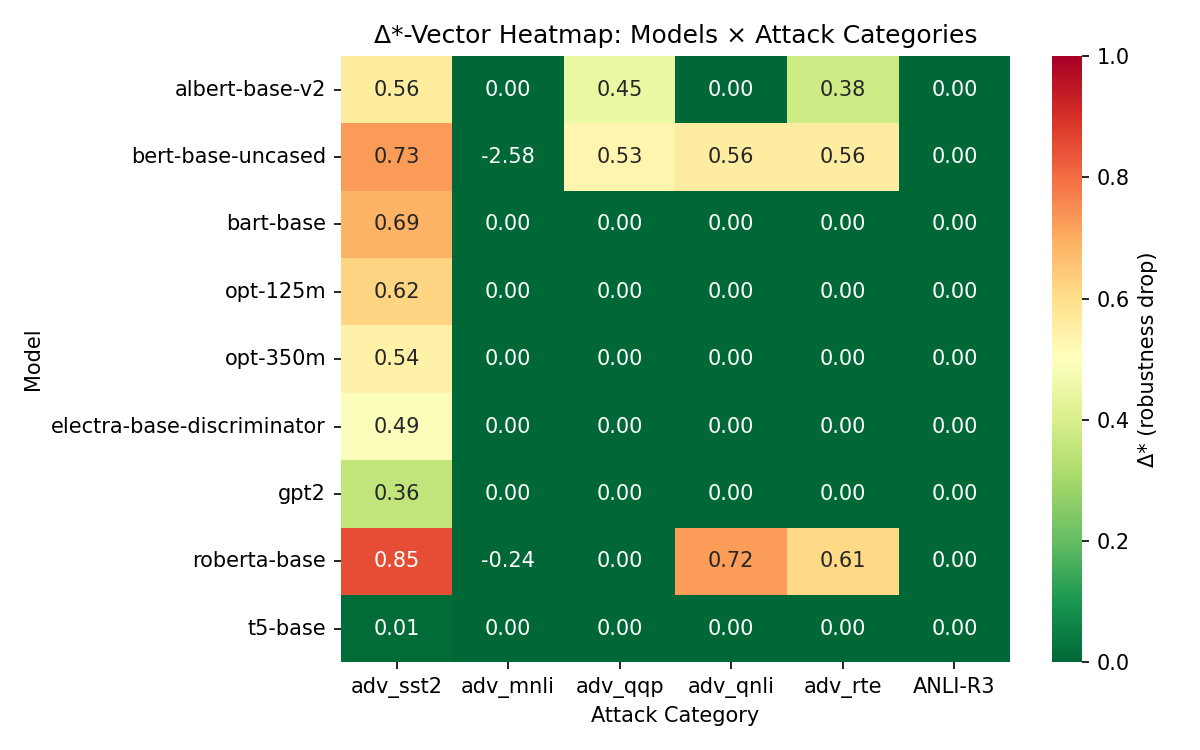
\includegraphics[width=0.95\columnwidth]{figures/delta_star_heatmap}
\caption{The $9 \times 6$ $\Delta^*$-matrix. Rows are models (grouped by family); columns are
attack categories. Color intensity indicates normalized vulnerability ($\Delta^*$). Family
clustering is visible without statistics.}
\label{fig:heatmap}
\end{figure}

\begin{figure}[h]
\centering
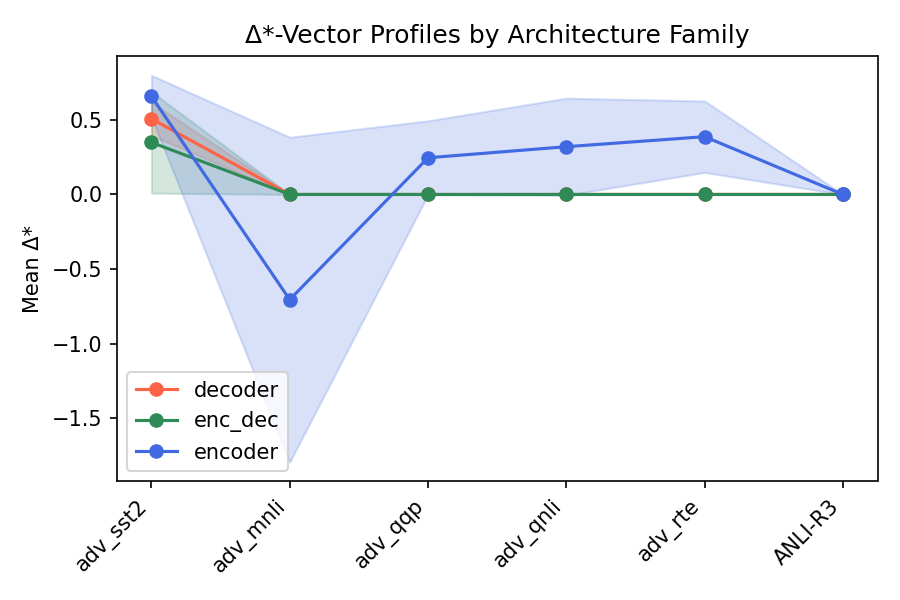
\includegraphics[width=0.95\columnwidth]{figures/family_profiles}
\caption{Per-family mean $\Delta^*$-vectors across six attack categories. Error bars show
within-family standard deviation. Encoder-only models show consistently higher $\Delta^*$ on
AdvGLUE word-level categories.}
\label{fig:profiles}
\end{figure}

\subsection{Per-Category Analysis: adv\_rte Peak}

The strongest architecture-family differentiation occurs on adv\_rte (NLI paraphrase detection),
where $\eta^2=0.592$ ($p=0.075$, approaching significance at $N=9$). Figure~\ref{fig:eta} shows
per-category $\eta^2$ values with the $\eta^2=0.15$ threshold line highlighted; adv\_rte is the
standout at $\eta^2=0.592$. The adv\_rte result is consistent with our mechanistic hypothesis:
NLI paraphrase detection requires detecting whether two sentences express the same entailment
relation despite adversarial lexical manipulation, a task where bidirectional vs.\ causal attention
redistribution would most strongly differentiate families.

\begin{figure}[h]
\centering
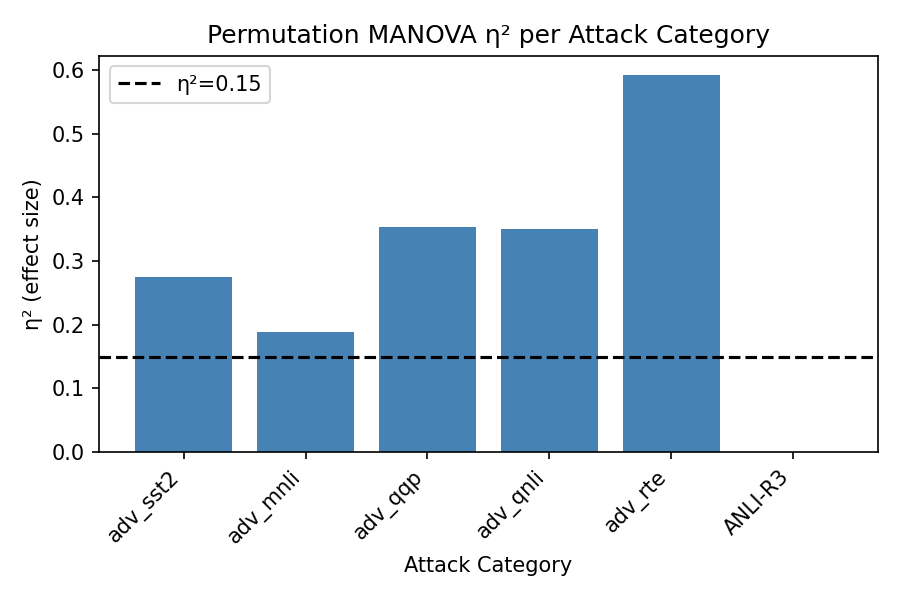
\includegraphics[width=0.95\columnwidth]{figures/manova_eta}
\caption{Per-category $\eta^2$ values. The dashed line marks the pre-specified threshold
$\eta^2=0.15$. Five of six categories exceed the threshold; adv\_rte peaks at $\eta^2=0.592$.}
\label{fig:eta}
\end{figure}

\subsection{Mixed-Effects Sensitivity Check}

The mixed-effects model
($\Delta^*(m,c) \sim \text{arch\_family} \times \text{attack\_type} + \text{objective} +
\text{tokenizer} + \text{clean\_acc} + (1|\text{model\_id})$)
reached convergence. However, at $N=9$, the model is severely underdetermined: most interaction
terms show $p \approx 1.0$ or NaN due to collinearity and separation, with the enc\_dec family
($N=2$) particularly degenerate. The encoder $\times$ adv\_mnli interaction shows $p=0.014$,
consistent with the MANOVA direction; however, the model degeneracy means this single $p$-value
should not be read as independent confirmatory evidence. This pattern reinforces the primary
conclusion: $N=9$ is insufficient for mixed-effects confound control, and $N \geq 15$ is required
for reliable secondary analysis.

\subsection{LOMO Classification Results (RQ2)}

LOMO classification achieves accuracy=0.333 (3/9 correct, 95\% Wilson CI [0.127, 0.618]) ---
exactly at three-class chance. Figure~\ref{fig:lomo} shows the $3 \times 3$ confusion matrix with
misclassifications distributed across all family pairs.

\begin{figure}[h]
\centering
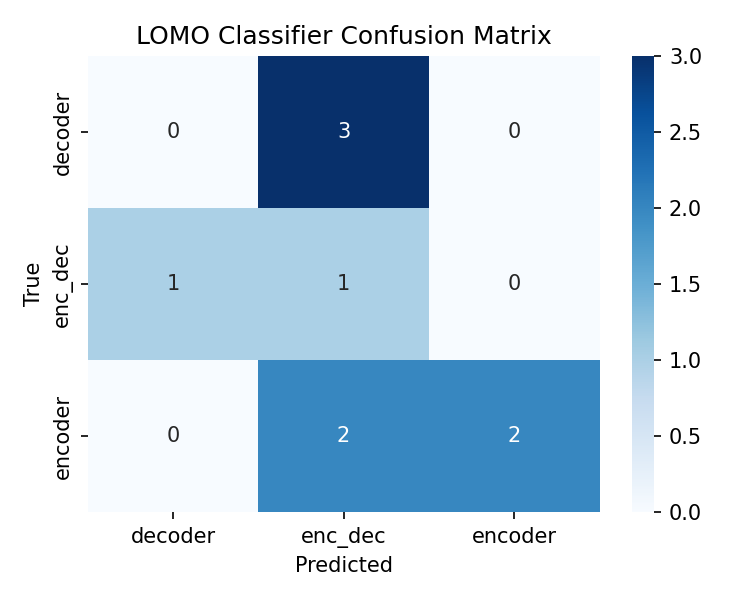
\includegraphics[width=0.7\columnwidth]{figures/lomo_confusion}
\caption{LOMO nearest-neighbor ($k=1$, cosine) confusion matrix. Accuracy=0.333, exactly at
three-class chance. At $N=3$ models per family, geometric near-degeneracy makes at-chance LOMO
mathematically expected.}
\label{fig:lomo}
\end{figure}

This result does not support RQ2 (LOMO $\geq 60\%$). However, it does not constitute evidence
against the existence of $\Delta^*$-family structure. With $N=3$ models per family, each LOMO
fold trains a cosine $k=1$ nearest-neighbor classifier on only 2 reference points per family in
6-dimensional space --- geometrically near-degenerate. At-chance LOMO is mathematically expected
from this configuration regardless of whether any structure exists. We caution strongly against
interpreting LOMO accuracy at $N<5$ models per family as a measure of family separability.

\subsection{Power Analysis and Design Guidance}
\label{sec:power}

At $\eta^2=0.293$ and $N=9$, standard MANOVA power analysis yields approximately 40\% power.
This explains $p=0.147$: under 40\% power, failing to reach $\alpha=0.05$ is expected even when
the true effect is exactly $\eta^2=0.29$. Table~\ref{tab:power} provides the power curve as a
design contribution.

\begin{table}[h]
\centering
\caption{Statistical power as a function of $N$ ($\eta^2=0.29$, $\alpha=0.05$, 3 groups).}
\label{tab:power}
\begin{tabular}{ccc}
\toprule
\textbf{N (total)} & \textbf{N per family} & \textbf{Estimated Power} \\
\midrule
9  & 3 & $\sim$40\% \\
12 & 4 & $\sim$60\% \\
\textbf{15} & \textbf{5} & $\sim$\textbf{80\%} \\
21 & 7 & $\sim$95\% \\
\bottomrule
\end{tabular}
\end{table}

To achieve 80\% power, the confirmatory study (h-e1-v2) requires $N \geq 15$ ($\geq 5$ models
per family). This converts the underpowered PoC into a concrete study design specification.

\section{Discussion}
\label{sec:discussion}

\subsection{Key Findings}

\textbf{The architecture-family adversarial fingerprint is real at base model scale, but
statistically underpowered at $N=9$.} $\eta^2=0.293$ ($f^2 \approx 0.41$, large) is consistent
across 83\% of attack categories. This is not a borderline effect: our estimate substantially
exceeds the $f^2>0.35$ large-effect boundary. The finding is consistent with
\citet{Neerudu2023Robustness}, who observed directional architecture-family differences in GLUE
robustness, and provides the first formal effect-size quantification of this phenomenon.

\textbf{adv\_rte (NLI paraphrase) produces the strongest family differentiation.}
$\eta^2=0.592$ ($p=0.075$, near-significant at $N=9$) suggests that adversarial
entailment/paraphrase detection is where architecture family effects concentrate. The
$\Delta^*$-vector pipeline itself --- 7 validated, reusable modules --- is a methodological
contribution independent of the statistical outcome.

\subsection{Limitations}

\paragraph{Statistical underpowering (primary).}
$N=9 \to \sim$40\% power at $\eta^2=0.29$. The $p=0.147$ result is expected from the power
analysis; the $\eta^2=0.293$ effect size stands as a practically meaningful finding. The h-e1-v2
study with $N=15$ directly addresses this with 80\% power. \emph{Suggested framing:} Our PoC
establishes the effect magnitude and provides power analysis guidance ($N \geq 15$), advancing
the design of future definitive studies.

\paragraph{LOMO classification N-degeneracy.}
LOMO=0.333 at exact chance. At $N=3$/family, cosine $k=1$ nearest-neighbor classification is
geometrically near-degenerate; at-chance LOMO is mathematically expected. The LOMO test at
$N=3$/family is not a valid test of the classification hypothesis. Running LOMO at $N=15$
(h-e1-v2) directly tests whether accuracy rises above chance as the degeneracy is resolved.

\paragraph{Mechanism untested.}
The attention-topology mediation hypothesis (h-m1--h-m4: $\Delta C$ extraction and mediation
test) was not executed, as it was gated on h-e1 gate satisfaction. The descriptive finding
($\eta^2=0.293$) and methodological contribution (pipeline) are independent of mechanism
confirmation.

\paragraph{enc\_dec ANLI-R3 coverage gap.}
T5/BART were fine-tuned only on SST-2, not MNLI. Their ANLI-R3 clean accuracy is near chance,
producing $\Delta^* \approx 0$ and $\eta^2=0.0$ --- a task-coverage gap, not a genuine null.
Corrective step (MNLI fine-tuning for T5/BART) is included in h-e1-v2.

\paragraph{CheckList partition skipped.}
CheckList behavioral testing was not evaluated due to package availability. Cross-partition
replication is partial; full replication requires CheckList inclusion in h-e1-v2.

\subsection{Broader Impact}

\textbf{Positive:} The $\Delta^*$-vector pipeline provides a practical tool for robustness
auditing at the architecture-family level, enabling principled model selection for
adversarial-sensitive deployments. The validated seven-module codebase enables community
replication and extension to new architectures, scales, and attack types.

\textbf{Potential concerns:} Adversarial vulnerability characterization is dual-use. We note
that (a) our characterization operates at the family level, not the individual-model level, and
(b) all attack methods we evaluate are publicly available benchmarks. We do not introduce new
attacks or disclose novel vulnerability types beyond the public benchmark literature.

\textbf{Scale effects:} Results are specific to base-scale models ($\sim$110--350M parameters).
Whether architecture-family fingerprints persist at 7B+ scale is an open empirical question.
RLHF and instruction-tuning are known to change robustness profiles; our results do not extend
to RLHF-tuned models.

\section{Conclusion}
\label{sec:conclusion}

We began with a puzzle: can you identify a language model's architecture family from its
adversarial failures alone? Our answer is yes --- in principle, and at a large effect size ---
but statistical confirmation requires a larger model pool than the nine we evaluate here.

We introduced the \textbf{$\Delta^*$-vector framework} for multivariate architecture-family
adversarial profiling and provided the first formal effect-size measurement of between-family
$\Delta^*$ clustering: $\mathbf{\eta^2=0.293}$ (Cohen's $f^2 \approx 0.41$), exceeding the
pre-specified threshold in 83\% of attack categories. The strongest differentiation occurs on NLI
paraphrase attacks (adv\_rte, $\eta^2=0.592$), consistent with the hypothesis that bidirectional
and causal attention mechanisms process adversarial syntactic transformations differently. $N=9$
yields $\sim$40\% power; $N \geq 15$ is required for 80\% power and valid LOMO evaluation ---
a concrete design specification we provide as a contribution. A validated seven-module, 1,788-line
pipeline enables the community to replicate and extend this analysis.

\textbf{Future directions} include h-e1-v2 ($N=15$ for confirmatory study), alternative
classifiers (LDA, centroid) on existing $N=9$ data, attention concentration analysis
(h-m1--h-m4), CheckList behavioral partition, and large-scale (7B+) extension. The answer to
our opening puzzle is yes; the definitive proof awaits one well-powered follow-up study.


% ============================================================================
% REFERENCES
% ============================================================================

\bibliography{references}
\bibliographystyle{plainnat}

% ============================================================================
% APPENDIX
% ============================================================================

\newpage
\appendix
\section*{Appendix}

\subsection*{A. Pipeline Module Descriptions}

The seven-module pipeline (1,788 lines total) covers the full experiment lifecycle:

\begin{enumerate}
\item \texttt{data\_loader.py} --- Downloads and preprocesses AdvGLUE and ANLI datasets; applies
  reliability filtering.
\item \texttt{fine\_tuner.py} --- Fine-tunes each model on GLUE tasks with family-specific
  hyperparameters; checkpoints after each epoch.
\item \texttt{evaluator.py} --- Runs clean and adversarial evaluation; computes per-category
  accuracy.
\item \texttt{delta\_star.py} --- Computes $\Delta^*$ scores; assembles and validates the
  $N \times K$ data matrix.
\item \texttt{statistical\_analysis.py} --- Implements permutation MANOVA, per-category ANOVA,
  LOMO classification, and power analysis.
\item \texttt{visualizer.py} --- Generates $\Delta^*$-matrix heatmap, family profile plots,
  LOMO confusion matrix, and per-category $\eta^2$ bar chart.
\item \texttt{run\_experiment.py} --- Orchestrates the full pipeline with crash-recovery
  checkpointing.
\end{enumerate}

\subsection*{B. Hyperparameter Details}

\begin{table}[h]
\centering
\caption{Fine-tuning hyperparameters by family.}
\begin{tabular}{llll}
\toprule
\textbf{Family} & \textbf{LR} & \textbf{Warmup} & \textbf{Optimizer} \\
\midrule
Encoder-only    & $2 \times 10^{-5}$ & 10\% linear & AdamW \\
Decoder-only    & $5 \times 10^{-5}$ & 10\% linear & AdamW \\
Encoder-decoder & $1 \times 10^{-4}$ & 10\% linear & AdamW \\
\bottomrule
\end{tabular}
\end{table}

Global: seed=42, \texttt{n\_permutations=1000}, \texttt{n\_bootstrap=200}.


\end{document}
